\chapter{Banco de pruebas}

En esta última sección nos dedicaremos a explicar algunos aspectos relevantes acerca del banco de pruebas que se ha desarrollado. Como se ha indicado anteriormente, la finalidad de este trabajo fin de grado no era la del desarrollo de una aplicación que se pudiera usar para el proceso digitalizado 3D sino del estudio de las ventajas e inconvenientes de cada uno de los métodos que intervienen. Por ello, esta aplicación ha sido una herramienta más usada durante el proceso. Sin embargo, se ha considerado que merece tener cierta atención ya que se han implementado algunas características interesantes, especialmente las relacionadas con las nubes de puntos, así como aspectos importantes de la Informática Gráfica. Por eso, no se va a hacer un estudio detallado acerca de la aplicación pero sí se van a explicar aspectos generales de la misma. \\

Para el desarrollo del programa ha sido de gran ayuda la referencia \cite{QT+Opengl}. En él se explica cómo desarrollar aplicaciones haciendo uso de la biblioteca \textit{OpenGL} (\textit{Open Graphic Library}) para el ámbito gráfico y \textit{C++} como lenguaje de programación. Sin embargo, la ventaja la encontramos en que utiliza la herramienta \textit{Qt}. La biblioteca gráfica solo nos permite producir los gráficos. Por ello, necesitamos una interfaz de usuario que nos permita la interacción y esa es la razón de usar \textit{Qt}. A modo aclaratorio, también es necesario el uso de \textit{GLEW} (\textit{OpenGL Extension Wrangler Library}) que nos permite una gestión más fácil de \textit{OpenGL}. También es conveniente destacar que el sistema operativo en el que se ha llevado a cabo todo este trabajo ha sido \textit{Ubuntu 18.04.4} sobre un ordenador con procesador \textit{Intel Core i7-3537U} y tarjeta gráfica \textit{GeForce GT 720M}.\\

Finalmente, notamos que la aplicación que se propone en \cite{QT+Opengl} ha servido como base para nuestro estudio. Principalmente, para el manejo de los diferentes objetos y algunos mecanismos como la selección de un punto (\textit{picking}). El código se ha ido completando y modificando según las necesidades que teníamos en cada etapa del desarrollo.

\begin{figure}
	\centering
	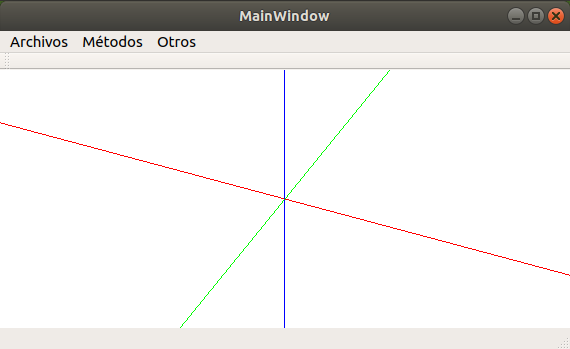
\includegraphics[width=0.7\linewidth]{banco/UI}
	\caption{Interfaz de usuario del banco de pruebas programado.}
	\label{fig:ui}
\end{figure}


\section{Estructura básica de la aplicación}\label{sec:estrucBasic}
Una vez se han explicado las herramientas con las que trabajamos, la aplicación base para la visualización consta de las siguientes clases:

\begin{itemize}
\item \textit{main}: es el programa principal. Su única finalidad es mostrar la ventana de la aplicación.
\item \textit{mainwindow}: es la encargada de crear la interfaz de usuario. Deriva a su vez de la clase \textit{QMainWindow}. En el archivo \textit{mainwindow.ui} encontramos almacenada la información relativa a su configuración, principalmente, los menús con los que iremos activando cada una de las funciones necesarias. 
\item \textit{\_gl\_widget}: clase derivada de \textit{QOpenGLWidget} y que implementa las funciones para dibujar con \textit{OpenGL}. Destacamos las funciones \textit{initializeGL}, \textit{resizeGL} y \textit{paintGL} que sirven para iniciar \textit{OpenGL}, actualizar el tamaño de la ventana y dibujar respectivamente. El código está preparado para visualizar los vértices, aristas o con relleno. Sin embargo, al trabajar nosotros con nubes de puntos, solo se visualizarán los mismos.
\end{itemize}

También se han programado los \textit{shaders}. A modo aclaratorio, estos programas se ejecutan en la tarjeta gráfica del juego (no en la CPU) y que se aplican para transformar vértices, aplicar iluminación o crear algún tipo de efecto. Existen dos diferentes: \textit{vertex shader} que se aplica para cada vértice y que transforma vértices, normales, calcula iluminación, etc. y \textit{fragment shader} para cálculo de color de un fragmento (información para generar un píxel). En nuestro caso se han programado, por un lado, los dos \textit{shaders} para la visualización normal de los objetos, y otro para la selección de puntos o \textit{picking} que en la sección \ref{sec:picking}.\\

En cuanto al manejo de la cámara, se hace mediante teclado siendo posible tanto acercar o alejar la cámara y rotarla para observar mejor la imagen. La cámara se mueve alrededor de una esfera con centro el origen y no se ha añadido la posibilidad de cambiarlo. Por ello, es posible que haya objetos que podamos visualizar bien debido a su situación en el espacio. Esto se ha solucionado con la posibilidad de modificar la matriz de modelado de los mismos (mediante combinación de teclas). Esta matriz, como se ha indicado al final del capítulo anterior, se aplica a cada uno de los vértices del modelo y sirve para posicionarlos. Por ejemplo, cuando es la identidad, los puntos se mantienen en las mismas coordenadas que indican sus vértices. Sin embargo, si componemos transformaciones (en nuestro caso traslaciones pero también se puede hacer con cualquiera) a la misma conseguimos desplazar o escalar el objeto sin añadir carga extra. Esto se debe en el propio \textit{vertex shader} se utiliza para calcular la posición de los puntos, junto las matrices de proyección y vista (ver sección \ref{sec:selecRec}). \\

También relacionada con evitar demasiada carga de trabajo a la aplicación, nos encontramos con la manera de enviar los vértices a la tarjeta gráfica. Nos encontramos que estamos trabajando con una gran cantidad de puntos por lo que necesitamos que este trabajo se haga de manera rápida. Para solventar este inconveniente se usa el \textit{envío en diferido} de los datos mediante los llamados \textit{Vertex Buffer Object} (VBO). Estos son vectores que solo pueden ser usados por las tarjetas gráficas. Esto implica que los datos que necesitamos, vértices y colores, se encuentren en la GPU (\textit{Graphics Processing Unit}) en vez de en memoria principal, acelerando el proceso de lectura de los mismos. Estos se han agrupado en un \textit{Vertex Array Object} (VAO), que básicamente son estructuras para almacenar VBOs y que los activa autáticamente. \\

Dentro del mismo VBO almacenamos la información relativa a diversos objetos. Por ello, necesitamos saber en cada momento qué posición ocupa cada uno de esos objetos para poder, por ejemplo, visualizar algunos de ellos. Es ahora cuando entra en juego la clase \textit{\_object\_management}. Esta clase contiene todos los objetos de la escena y se encarga del manejo de las posiciones de inicio dentro del vector y del tamaño de cada uno de los mismos. \\

\subsection{Clase \textit{\_basic\_object3D}}
La clase que representa un objeto genérico es \textit{\_basic\_object3D}. Encontramos por ejemplo los vértices, colores, normales, puntos claves, etc. Se ha ido modificando según las necesidades que teníamos en cada momento. Destacamos que de esta clase deriva otra, \textit{\_malla\_ptx} que es la encargada de guardar y leer objetos que vienen en un archivo con formato PTX. \\

Destacamos que los puntos se mantienen en dos vectores y en una matriz. Un primer vector, que podríamos considerar auxiliar, con solo los vértices y que es el que se utiliza para rellenar el VBO. El segundo y la matriz contienen elementos de una estructura que hemos definido y que se denomina \textit{Punto}. Contiene tanto las coordenadas del vértice así como información relevante del mismo: posición dentro de la matriz (en el caso del vector) o del vector (en el caso de la matriz) y si el punto está activo o no. El hecho de hacerlo se debe a que cada uno de los casos es beneficioso para unas operaciones u otras. La matriz es la que nos indica la relación de vecindad entre cada uno de los puntos. Se usa, por ejemplo, para acelerar el cálculo de las normales, ya que solo tenemos que acceder a las posiciones de la matriz que rodean al vértice actual y no es necesario buscarlas en el vector de vértices. Por otro lado, el vector es más intuitivo a la hora del manejo de vértices en general. En cuanto a si al punto se encuentra activo o no se refiere a si se ha borrado o no. Al realizar una toma, generalmente no se capta solamente el objeto deseado en sí, sino también parte de su entorno. Así, necesitamos indicar los puntos que no nos interesan (ver sección \ref{sec:selecRec}) y borrarlos. En vez de ir modificando el vector de vértices dejando solo los activos, lo que conllevaría una gran carga de trabajo al escribir constantemente en memoria, solo se marca si un vértice está activo o no. De este modo, una vez se tienen marcados los que se quieren visualizar, solo se tiene que actualizar el vector que utiliza el VBO. En cuanto a los colores de cada vértice, tenemos también dos vectores como en el caso de los vértices: uno con todos los colores (tanto de vértices activos como no activos) y otro que se envía a la GPU.\\

Es interesante destacar las funciones para leer y guardar los archivos, sobre todo esta última. Cuando hemos modificado un objeto, ya sea porque hemos alterado su posición o hemos eliminado puntos, necesitamos mantener las relaciones de vecindad del conjunto que teníamos originalmente (para poder calcular las normales, por ejemplo). También, para el caso de que se hayan borrado puntos, el archivo que contiene el modelo modificado debería ocupar menos espacio. Por eso, para guardar, lo que hacemos es encontrar la mínima matriz que contiene a todos los vértices activos y solo guardar dichas filas y columnas. Es posible que esta submatriz contenga puntos que no estén activos. Como no es posible guardar dicha información en el formato PTX, que es con el tipo de datos que estamos trabajando, se ha optado por darle unas coordenadas a esos vértices muy alejadas. Así, al leer el modelo, vemos si la distancia de cada vértice al origen está dentro de una cota. Si no la cumple, marcamos el vértice como no activo y no se dibujaría, pero se seguiría manteniendo la coherencia espacial. Esta cota también la podemos utilizar para filtrar directamente puntos al cargar un archivo y ahorrarnos el eliminarlos manualmente (ver figura \ref{fig:filtrado}). Al cargar también tenemos en cuenta otro parámetro que nos aporta el formato PTX: el coseno del ángulo de incidencia en el plano. De este modo, solo nos quedamos con aquellos puntos que no estén muy oblicuos, ya que eso implica mayor error en la toma de la muestra. Tanto estos valores de filtrado como los de los algoritmos se han pasado al programa mediante lectura de ficheros. Apuntar que el simplificado de las mallas  que hemos mencionado en capítulos anteriores, se hace igual que la operación de guardar, solo aumentamos en cada iteración el incremento del índice para recorrer la matriz.  \\

\begin{figure}[h!]
	\begin{minipage}{0.5\textwidth}
		\centering
		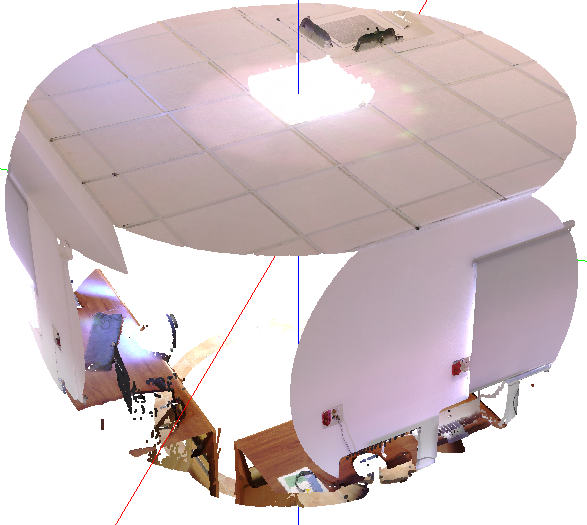
\includegraphics[width=1\linewidth]{banco/filtrado1} 
		\caption*{(a)}
		%\label{fig:subim1}
	\end{minipage}
	\begin{minipage}{0.5\textwidth}
		\centering
		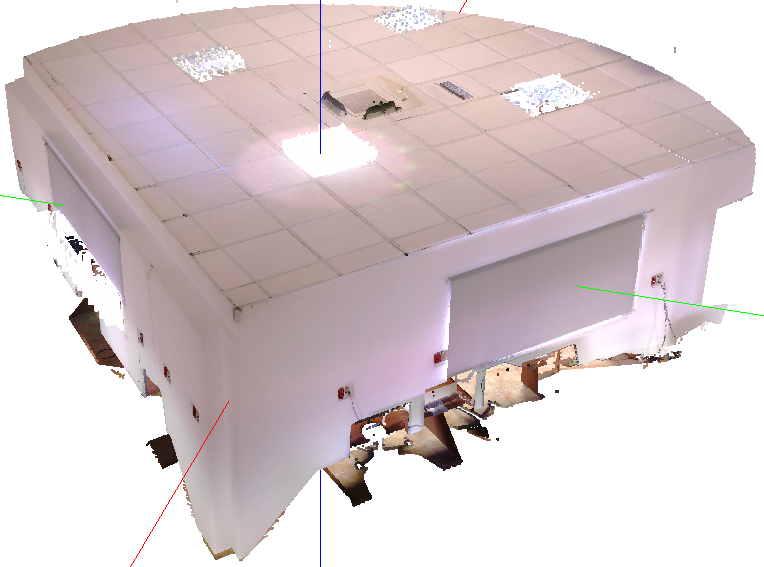
\includegraphics[width=1\linewidth]{banco/filtrado2} 
		\caption*{(b)}
		%\label{fig:subim1}
	\end{minipage}
	\caption{Ejemplo de filtrado según la distancia al escáner al cargar un modelo: (a) filtrado a 2 metros y (b) filtrado a 4 metros.}
	\label{fig:filtrado}
\end{figure}

Esta clase proporciona los funciones con los métodos de alineado que hemos estudiado. Destacamos que los procesos se han ido dividiendo en etapas. Esto se debe a que lo que nos interesaba era conocer el proceso en sí y no tanto tener un único mecanismo para hacerlo completo. Por eso, en ICP tenemos tanto la función de prealineado junto con otra para ejecutar solamente un paso del algoritmo (aunque también hay una función para ejecutar varias iteraciones con condición de parada la original y un número máximo de iteraciones si fuese necesario). Por su parte, el proceso de RANSAC se ha dividido a su vez en el cálculo de planos, poder cargarlos a partir de un archivo, cálculo de intersecciones entre los mismos, etc. Esta división también facilita las tareas de depuración, ya que tenemos cada tarea por separado así como poder reproducir los resultados una vez tenemos calculados correctamente algunos datos.

\section{Picking}\label{sec:picking}
Esta sección junto con la siguiente podemos considerar que son más interesantes dentro del ámbito de la Informática Gráfica. El \textit{picking} consiste en seleccionar un único elemento de la escena. En nuestra aplicación, queremos seleccionar los vértices para el proceso de prealineado. Este proceso debe ser tanto rápido como interactivo. Por ello, una de las soluciones más usadas para solucionar este problema es la llamada \textit{selección por color}. Este método consiste en tener un identificador único para cada elemento y convertirlo de manera unívoca en un color. De este modo, podemos pasar de identificador a color y viceversa sin ningún tipo de problemas. Así, lo único que hay que hacer es dibujar el objeto con estos colores modificados, obtener el color de la posición que se ha seleccionado y recuperar el identificador. Como un color en RGB (\textit{Red Blue Green}) se representa mediante tres bytes, tenemos un total de $ 16\,777\,216 $ de combinaciones. A esta cantidad habría que quitarle la combinación del blanco que se utiliza para indicar que no se ha seleccionado nada. \\

La relación entre identificador y color es de la siguiente manera:
\begin{itemize}
	\item Identificadores de 0 a 255 van a la componente azul.
	\item Identificadores de 256 a $ 65\,535 $ van a la componente verde.
	\item Identificadores de $ 65\,535 $ a $ 16\,777\,215 $ van a la componente roja.
\end{itemize}

Esta conversión se hace fácilmente mediante máscaras y rotaciones de los bits. Ya tenemos la manera de asociar colores e identificadores, ahora, ?`cuál es el identificador para cada vértice que vamos a usar?. Usaremos la posición que ocupa cada vértice en el vector del VBO y que nos lo aporta directamente la directiva \textit{gl\_PrimitiveID} del \textit{fragment shader}. Como se ha mencionado en \ref{sec:estrucBasic} necesitamos por tanto otro programa \textit{shader} diferente: en el \textit{vertex} solo calculamos la posición en el mundo de cada vértice y en el \textit{fragment} hacemos la conversión de identificador a color. \\

Volviendo al proceso, hemos comentado que tenemos que dibujar el objeto con los nuevos colores asignados. Esto no lo podemos hacer en la pantalla, ya que ahí queremos visualizar el objeto normal. Si se hiciese de ese modo se observaría un parpadeo. Se utiliza entonces un \textit{framebuffer}, esto es, una zona de memoria donde se dibuja la imagen y se hacen otras operaciones como el cálculo de las profundidades (algorimto \textit{z-buffer}). El \textit{framebuffer} principal es el único que permite mostrar por la pantalla por lo que debemos crear uno propio, asignándole tanta zona de memoria para los colores como otra para el \textit{z-buffer}. Finalmente, solo falta obtener el color del pixel seleccionado mediante la función \textit{glReadPixels}. En la figura \ref{fig:shaders}, encontramos un ejemplo de visualización normal y otras con los colores para el \textit{picking}.

\begin{figure}[h!]
	\begin{minipage}{0.5\textwidth}
		\centering
		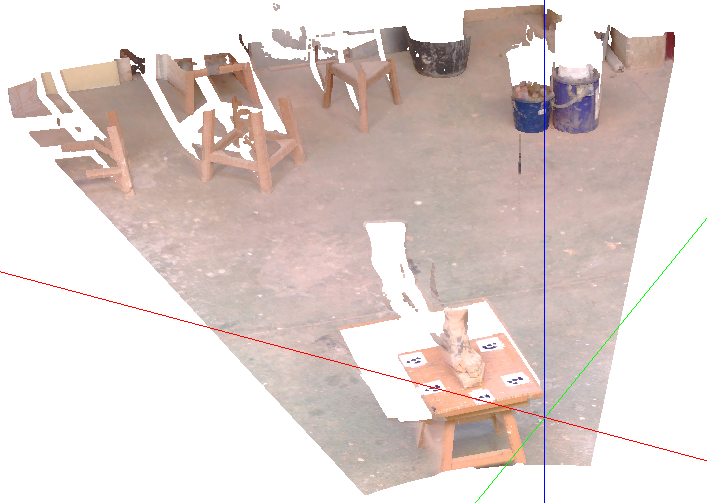
\includegraphics[width=1\linewidth]{banco/pick1} 
		\caption*{(a)}
		%\label{fig:subim1}
	\end{minipage}
	\begin{minipage}{0.5\textwidth}
		\centering
		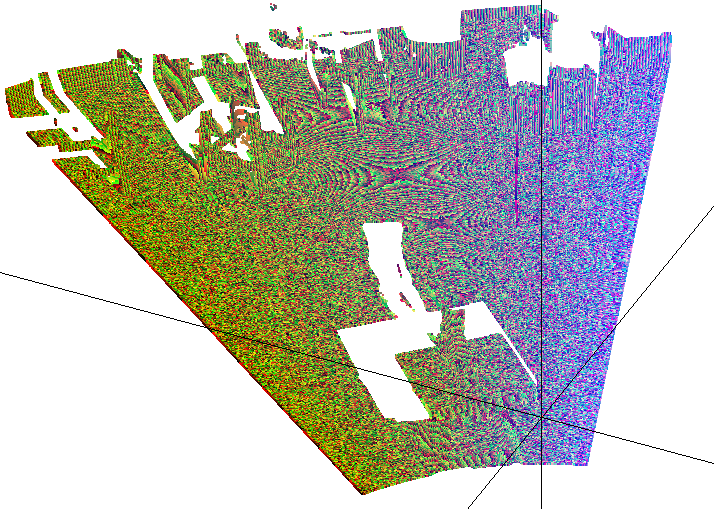
\includegraphics[width=1\linewidth]{banco/pick2} 
			\caption*{(b)}
		%\label{fig:subim1}
	\end{minipage}
	\caption{Visualización con los dos programas \textit{shader}: (a) visualización normal y (b) visualización con la asignación de colores según identificador para el picking}
	\label{fig:shaders}
\end{figure}

\section{Selección mediante rectángulo}\label{sec:selecRec}
Otra de las funciones a nombrar y que se han incluido en el banco de pruebas es la posibilidad de seleccionar puntos mediante un rectángulo. Esto es clave para eliminar las partes que no nos interesan de las tomas. Uno de los aspectos que involucra a este tema ya se ha explicado y es mantener la información de si un punto está activo o no para no elevar la carga dae trabajo. El segundo aspecto a destacar lo tratamos aquí es la propia detección de puntos que están dentro del rectángulo y que se ha abordado de manera diferente al \textit{picking}.\\

En primer lugar, necesitamos dibujar el propio rectángulo que indica la selección. Para ello se ha usado un objeto la clase \textit{QRubberBand} que proporciona \textit{Qt}. Además, ya tiene un método que nos proporciona si un determinado elemento está dentro del mismo o no. ?`Cuál es el aspecto interesante? Se trata del tipo de coordenadas que recibe como entrada dicha función y que veremos a continuación. \\

Para poder dibujar correctamente la figura en pantalla, hay que tener en cuenta no solo el lugar del objeto en el mundo virtual sino también la posición de la cámara, modificaciones en el propio objeto, etc. Esto ya se ha tratado al hablar de las traslaciones del objeto mediante modificaciones de la matriz de modelado, por ejemplo. Así, el flujo para obtener el lugar de la pantalla donde se proyecta cada vértice es el siguiente:

\begin{enumerate}
\item Los vértices vienen dados en coordenadas de objeto que es la posición según el marco de referencia del propio objeto.
\item Primero aplicamos la matriz de modelado para obtener las coordenadas del mundo que son comunes a toda la escena. 
\item A continuación, mediante la matriz de vista, se obtienen las coordenadas de ojo y que se puede ver como la transformación que nos sitúa en el marco de referencia de la cámara.
\item Una vez hecho esto, necesitamos recortar la imagen indicando la región que queremos que sea visible así como el tipo de proyección que queremos, en nuestro caso principalmente con perspectiva. Esto se hace mediante la matriz de proyección.

\begin{figure}[h!]
	\begin{minipage}{0.5\textwidth}
		\centering
		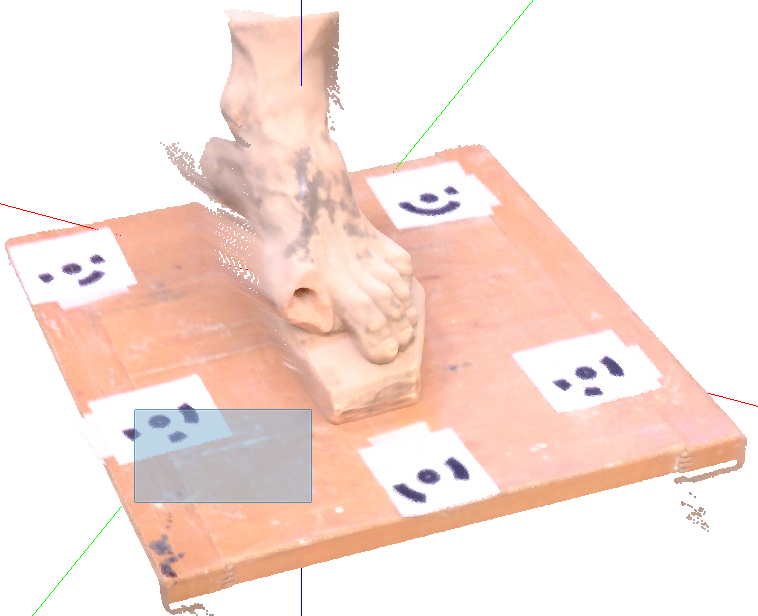
\includegraphics[width=1\linewidth]{banco/rect2} 
		\caption*{(a)}
		%\label{fig:subim1}
	\end{minipage}
	\begin{minipage}{0.5\textwidth}
		\centering
		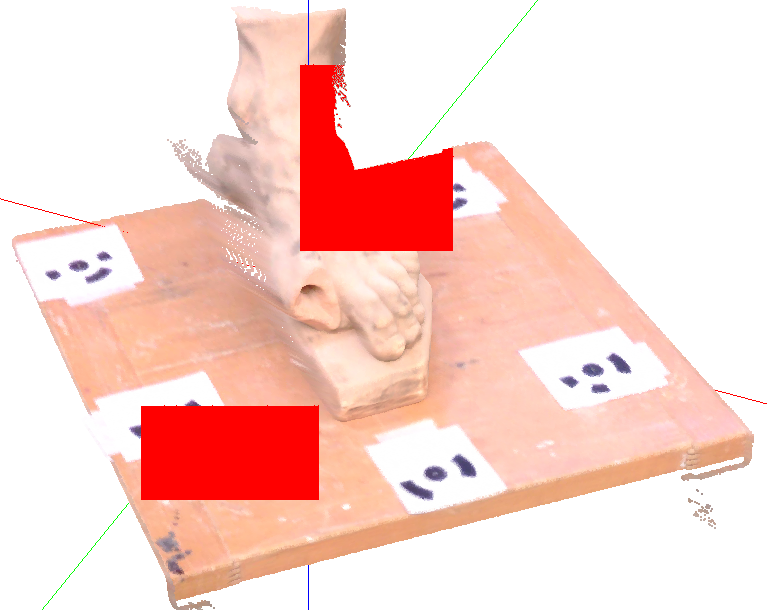
\includegraphics[width=1\linewidth]{banco/rect3} 
		\caption*{(b)}
		%\label{fig:subim1}
	\end{minipage}
	\begin{minipage}{0.5\textwidth}
		\centering
		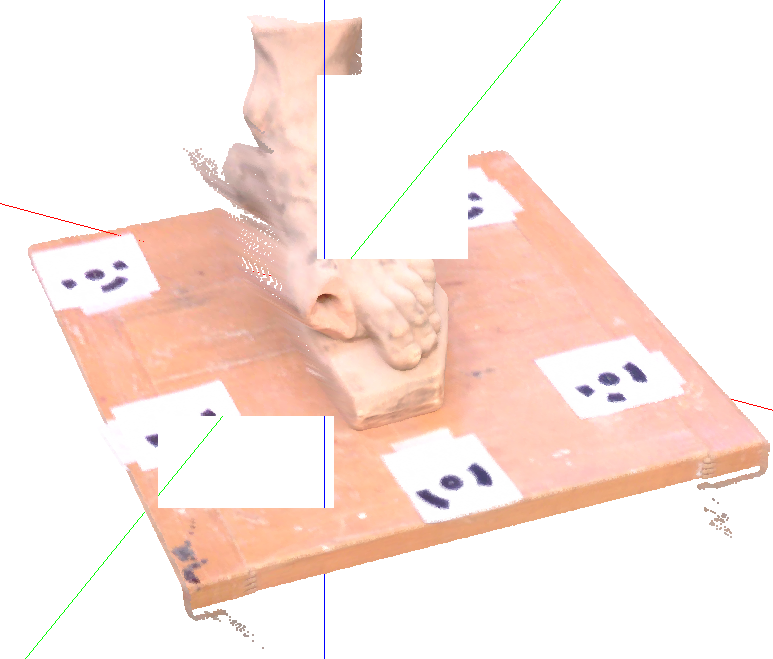
\includegraphics[width=1\linewidth]{banco/rect4} 
		\caption*{(c)}
		%\label{fig:subim1}
	\end{minipage}
	\begin{minipage}{0.5\textwidth}
		\centering
		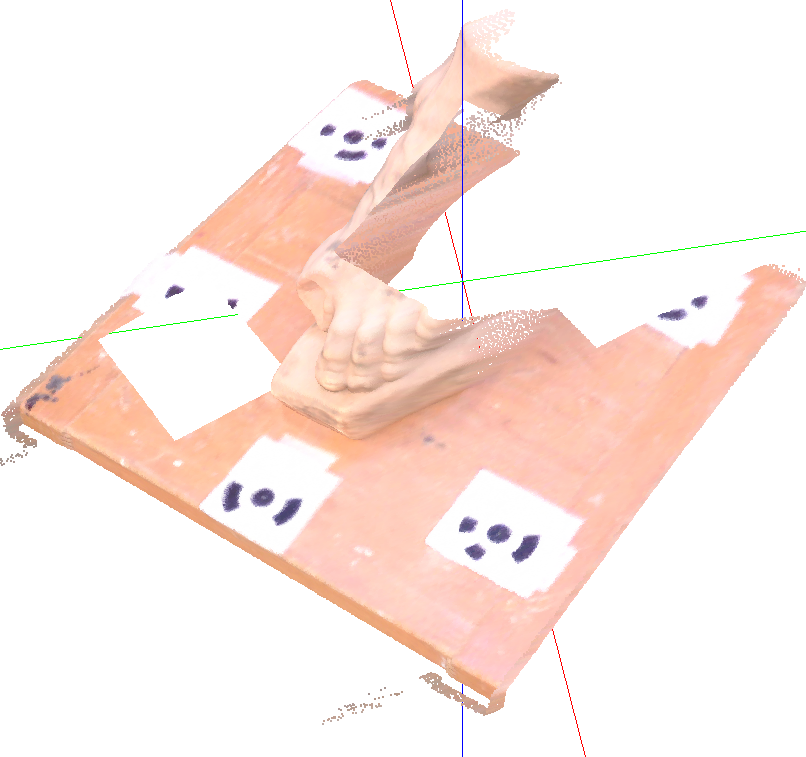
\includegraphics[width=1\linewidth]{banco/rect5} 
		\caption*{(d)}
		%\label{fig:subim1}
	\end{minipage}
	\caption{Borrado de puntos: (a) rectángulo de selección, (b) zona a borrar con posibilidad de mantener los seleccionados anteriores, (c) y (d) modelo tras borrar los puntos seleccionados.}
	\label{fig:delRect}
\end{figure}

\item A continuación se obtienen las coordenadas normalizadas de dispositivo, para que las coordenadas del punto se encuentren entre $ \left[-1,1\right] $. Esto se hace mediante la división de un cuarto parámetro que obtenemos directamente del paso anterior.
\item Por último, se tienen las coordenadas de dispositivo mediante la transformación lineal de llevar el intervalo $ \left[-1,1\right] $ al tamaño y posición del \textit{viewport} dentro de la ventana actual.

\end{enumerate}

Una vez explicado el proceso, notamos que las matrices de modelado y de vista son relativamente fáciles de calcular: la primera porque es resultado de transformaciones que hemos ido aplicando y para la segunda hay que tener en cuenta que la cámara viene dada en nuestro caso en coordenadas esféricas. En cuanto a la matriz de proyección, la podemos obtener directamente pasando los parámetros del área que queremos visualizar. Así, la función \textit{contains} de nuestro rectángulo recibe las coordenadas de dispositivo y que son necesarias calcularlas manualmente. En la figura \ref{fig:delRect} vemos un ejemplo de selección y borrado de un conjunto de puntos. \\

En definitiva, aunque el proyecto se haya centrado en otros aspectos, gracias al desarrollo de este banco de pruebas se han podido conocer nuevos entornos de desarrollo. También se han profundizado en otros aspectos relacionados con la informática  gráfica que en mayor o menor medida ya se habían estudiado anteriormente pero se ha considerado que eran lo suficientemente relevantes para volver a tratarlos. Además, se han debido de solucionar problemas, como guardar modelos modificados, que aunque no son relevantes en las conclusiones obtenidos, son de suma importancia a la hora de poder trabajar.


\section{Código, instalación y uso}
Los archivos correspondientes a la aplicación se encuentran dentro de la carpeta \textit{Banco de pruebas}. No hace falta realizar ningún tipo de instalación para poder ejecutar el banco de pruebas. En la documentación entregada se encuentra el archivo ejecutable denominado \textit{Application} que puede ser ejecutado directamente desde una terminal en \textit{Linux}. En la carpeta \textit{src} se encuentra el código del programa y en \textit{ES} están los distintos archivos auxiliares que hemos mencionado para pasar parámetros al programa. También, se adjunta un ejemplo de un modelo en formato PTX dentro de la carpeta \textit{Ejemplo}. Para cargarlo, seleccionamos en el menú la opción \textit{Archivos > Abrir}.\\

Para mover la cámara se usan las flechas del teclado y para acercar y alejar la misma se usan las teclas menos y más respectivamente. Destacar que las combinaciones te teclado para modificar la matriz de modelado son: \textit{CTRL+f} para mover al frente, \textit{CTRL+b} para mover atrás, \textit{CTRL+u} para mover arriba, \textit{CTRL+d} mover abajo, \textit{CTRL+l} mover a la izquierda y \textit{CTRL+r} mover a la derecha. Para activar la selección de puntos aislados usamos la tecla \textit{s} y para la selección por rectángulo \textit{r} (si mantenemos pulsado \textit{CTRL} podemos seleccionar varias zonas a la vez). Finalmente, para borrar los puntos seleccionados se usa la tecla \textit{d}. 



